% MASTER 1 -- Conducting slab / transistor channel (the "labeled rectangle" block).
% Sheet resistance R_S = rho/t ; R = R_S * (L/W) = (number of squares) * R_S.
% Covers Q1 (sheet-resistance derivation figure) directly.
% Reuse for Q10: it is the same rectangle -- just relabel as a channel with W=2*lambda
% and L=2*lambda (R=10k) or L=8*lambda (R=40k). Current flows along L.
\documentclass[border=10pt]{standalone}
\usepackage{amsmath}
\usepackage{tikz}
\usetikzlibrary{arrows.meta,calc}
\begin{document}
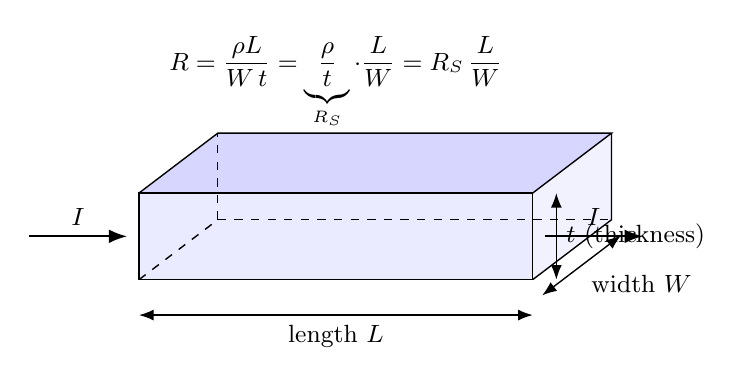
\begin{tikzpicture}[>=Latex,font=\small,line width=0.5pt]
  \def\Lx{5}    % length along current  (x)
  \def\Ty{1.1}  % thickness             (y, up)
  \def\Wd{2.0}  % width into the page   (depth)
  \def\sx{0.5}  % depth shear in x
  \def\sy{0.38} % depth shear in y
  % front face (L x t)
  \coordinate (fbl) at (0,0);
  \coordinate (fbr) at (\Lx,0);
  \coordinate (ftr) at (\Lx,\Ty);
  \coordinate (ftl) at (0,\Ty);
  % back face (shifted by depth W)
  \coordinate (bbl) at ($(fbl)+(\sx*\Wd,\sy*\Wd)$);
  \coordinate (bbr) at ($(fbr)+(\sx*\Wd,\sy*\Wd)$);
  \coordinate (btr) at ($(ftr)+(\sx*\Wd,\sy*\Wd)$);
  \coordinate (btl) at ($(ftl)+(\sx*\Wd,\sy*\Wd)$);
  % visible faces
  \fill[blue!8]  (fbl) -- (fbr) -- (ftr) -- (ftl) -- cycle;  % front
  \fill[blue!16] (ftl) -- (ftr) -- (btr) -- (btl) -- cycle;  % top
  \fill[blue!5]  (fbr) -- (bbr) -- (btr) -- (ftr) -- cycle;  % right
  % edges
  \draw (fbl)--(fbr)--(ftr)--(ftl)--cycle;
  \draw (ftl)--(btl)--(btr)--(ftr);
  \draw (fbr)--(bbr)--(btr);
  \draw[dashed] (fbl)--(bbl); \draw[dashed] (bbl)--(bbr); \draw[dashed] (bbl)--(btl);
  % current arrows along L
  \draw[->,thick] (-1.4,\Ty/2) -- (-0.15,\Ty/2) node[midway,above]{$I$};
  \draw[->,thick] (\Lx+0.15,\Ty/2) -- (\Lx+1.4,\Ty/2) node[midway,above]{$I$};
  % dimension labels
  \draw[<->] (0,-0.45) -- (\Lx,-0.45) node[midway,below]{length $L$};
  \draw[<->] (\Lx+0.30,0) -- (\Lx+0.30,\Ty) node[midway,right]{$t$ (thickness)};
  \draw[<->] ($(fbr)+(0.12,-0.20)$) -- ($(bbr)+(0.12,-0.20)$) node[midway,below right]{width $W$};
  % formula
  \node[align=center] at (\Lx/2,\Ty+1.4)
     {$R=\dfrac{\rho L}{W\,t}=\underbrace{\dfrac{\rho}{t}}_{R_S}\cdot\dfrac{L}{W}
       =R_S\,\dfrac{L}{W}$};
\end{tikzpicture}
\end{document}
